\documentclass{article}

\usepackage[left=1.5in, right=1.5in, top=1in, bottom=1in]{geometry}
\usepackage{amsmath}
\usepackage{amssymb}
\usepackage{hyperref}
\usepackage{graphicx}

\begin{document}

\begin{flushleft}

\section{Background Information}

Sources: \href{https://www.pnas.org/doi/full/10.1073/pnas.1416287112}{Boareto et al., 2015}, \href{https://www.nature.com/articles/nrm2009}{Bray, 2006}

\medskip

Binding of the Delta ligand from cell $B$ to the Notch receptor on cell $A$ results in the \emph{cleavage} (removal) of both the ligand and receptor. This interaction triggers the release of NICD (Notch Intracellular Domain) in cell $A$, which \emph{promotes} Notch and \emph{inhibits} Delta.

\begin{itemize}
  \item The Serrate (Jagged) ligand can also bind to Notch. Unlike Delta, NICD promotes Jagged, which creates a double-positive feedback loop.
  \item Interaction between Delta ligands and Notch receptors from the same cell (cis-interaction) removes both molecules and does not trigger the release of NICD.
\end{itemize}

\section{Ideas and Issues with Collier et al., 1996}

\subsection{Model}

Collier et al. make the following five modelling assumptions:
\begin{enumerate}
  \item Cells interact through Delta-Notch signalling if and only if they are adjacent.
  \item Production of Notch is an increasing (hill) function of Delta in neighbouring cells.
  \item Production of Delta is a decreasing (hill) function of Notch in the same cell.
  \item Production of Notch and Delta is balanced by decay proportional to concentration.
  \item Low levels of Notch cause the primary fate, high levels cause the secondary fate.
\end{enumerate}

Then they define the following variables:

\begin{itemize}
  \item $\tau$: time
  \item $N_{P}$: notch activity (concentration) in cell $P$
  \item $D_{P}$: delta activity (concentration) in cell $P$
  \item $\overline{D}_{P}$: average delta activity in neighbours of $P$
  \item $N_{0}$: typical notch activity (across all cells)
  \item $D_{0}$: typical delta activity (across all cells)
  \item $\mu$: The decay rate for notch (assumed constant)
  \item $\rho$: The decay rate for delta (assumed constant)
\end{itemize}

Then, define the following system of differential equations, where $F:[0, \infty) \rightarrow [0, \infty)$ is a continuous increasing function and $G: [0, \infty)\rightarrow [0, \infty)$ is a continuous decreasing function.

$$
\begin{aligned}
  \frac{d(N_{P} / N_{0})}{d\tau} = F(\overline{D}_{P} / D_{0}) - \mu N_{P} / N_{0} \\[5pt]
  \frac{d(D_{P} / D_{0})}{d\tau} = G(N_{P} / N_{0}) - \rho D_{P} / D_{0}
\end{aligned}
$$

This equation is inherently nondimensional, since $N_{P} / N_{0}$ and $D_{P} / D_{0}$ have no units.

\newpage

\subsection{Issues}

The Collier et al. model makes numerous simplifications that violate our current understanding of the delta-notch signalling network. These simplifications make it difficult to derive a probabilistic model from the Collier et al. model, since the biological implications of such a model would be contradictory. Some of the issues include:

\begin{itemize}
  \item Production of activated Notch (NICD) is exclusively a function of the Delta concentration in neighbouring cells, with no regard for the concentration of extracellular Notch receptors.
  \item Furthermore, the concentration of extracellular Notch isn't accounted for at all, which means there is no way to create a meaningful reaction term that captures the dynamics of the system.
  \item There are smaller issues, like the absence of cis-inhibition and the Serrate (Jagged) protein, but these aren't necessary to capture the fundamental behaviour of the system.
\end{itemize}

\subsection{Qualitative Results}

In the two-cell periodic boundary condition case, Collier et al. show that there always exists a homogeneous steady state, although this state is unstable if the feedback in the Delta-Notch signalling network is sufficiently strong. If the line of cells is given Dirichlet boundary conditions, the inhomogeneity arises on the outside edges before gradually spreading inwards to the center of the domain. On the two-dimensional hexagonal lattice, the system exhibits different ratios of primary to secondary fated cells depending on the parameters. In particular, Collier et al. observed ratios of $1/2$, $1/3$, $1/4$, $1/5$, and $1/6$.

\section{Probabilistic Models of Increasing Complexity}

\textbf{Idea}: Our first goal is to develop a probabilistic model based on a modern understanding of the biochemistry of the delta-notch signalling network. Then, we will use this model to attempt to replicate qualitative results from Collier et al. (1996).

\subsection{A First Model}

Assume \emph{a priori} (i.e. from previous research) the following, where $I$ is NICD:

\begin{itemize}
  \item Basal extracellular Notch ($N$) production has the form $H^{+}(I) = n_{m}I^2/(n_{0}^2 + I^2)$. 
  \item Basal extracellular Delta ($D$) production has the form $H^{-}(I) = d_{m}/(d_{0}^2 + I^2)$.
  \item Extracellular Notch and Delta have the same decay rate, $\gamma$.
\end{itemize}

Then, define the following parameters:

\begin{itemize}
  \item $N_{0}$ and $D_{0}$ are the maximum rates of Notch/Delta production.
  \item $k_{T}$ is the binding rate between extracellular Notch and Delta.
  \item $N_{ext}$ and $D_{ext}$ refer to the average Notch/Delta levels in neighbouring cells.
  \item $\gamma_{I}$ is the decay rate of NICD.
\end{itemize}

\newpage

Furthermore, we will assume that there is no cis-interaction and no Serrate ligand. This gives us the following set of chemical reactions that can occur in a single time step:

\begin{enumerate}
  \item A Notch receptor (from cell $A$) binds to a Delta ligand (from cell $B$), triggering the release of NICD in cell $A$. This can be written as $N_{A} + D_{B} \rightarrow I_{A}$. The probability of this event is $k_{T}N_{A}D_{B}$.
  \item A Notch receptor in cell $A$ decays ($N_{A} \rightarrow \emptyset$) with probability $\gamma N_{A}$.
  \item A Delta ligand in cell $A$ decays ($D_{A} \rightarrow \emptyset$) with probability $\gamma D_{A}$.
  \item A NICD molecule in cell $A$ decays ($I_{A} \rightarrow \emptyset$) with probability $\gamma_{I}I_{A}$.
  \item A Notch receptor in cell $A$ is produced ($\emptyset \rightarrow N_{A}$) with probability $H^{+}(I)$.
  \item A Delta ligand in cell $A$ is produced ($\emptyset \rightarrow D_{A}$) with probability $H^{-}(I)$.
\end{enumerate}

\subsection{Computational Implementation}

We will make the assumption that reaction times follow a Poisson point process. Let $E$ be the set of all possible reaction events (i.e. reactions 1-6 above for all cells). Furthermore, let $|E| = N$ be the number of possible reactions. For each event, let $X_{i} \sim \text{Exp}(\lambda_{i})$ denote the time until the next event of type $i$, where $1 \leq i \leq N$. Then, the waiting time $T$ in between \emph{any} two events is:

$$
T = \text{min} \{ X_{1}, \dots, X_{N} \} \sim \text{Exp}\left( \sum_{i = 1}^{N} \lambda_{i} \right) 
$$

This results follows from the definition of an exponential distribution and the memoryless property. Then, we can use Gillespie's algorithm to simulate the system as follows:

\medskip

\textbf{Step 1}: Sample a value $t_{i}$ from $T$ using inverse transform sampling. 

\medskip

\textbf{Step 2}: Increment the current time $t$ by $t_{i}$.

\medskip

\textbf{Step 3}: Determine which event took place. To do this, recall that:

$$P(X_{k} = \text{min} \{  X_{1}, \dots, X_{N} \}) = \frac{\lambda_{k}}{\lambda_{1} + \dots + \lambda_{N}}$$

Use this fact to partition the interval $[0, 1]$. Then sample $y_{i}$ from a $\text{Unif}(0, 1)$ distribution, identify its partition, and find the corresponding event.

\medskip

\textbf{Step 4}: Update the state based on the event determined in the previous step.

\subsection{Theoretical Justification}

In this section, we need to show that in expectation, the model above converges to the following system of ODEs (adapted from Boareto et al., 2015):

$$
\begin{aligned}
  \frac{dN}{dt} &= \frac{n_{m}I^2}{n_{0}^2 + I^2} - k_{T}ND_{ext} - \gamma N \\[5pt]
  \frac{dD}{dt} &= \frac{d_{m}}{d_{0}^2 + I^2} - k_{T}DN_{ext} - \gamma D \\[5pt]
  \frac{dI}{dt} &= k_{T}ND_{ext} - \gamma_{I}I
\end{aligned}
$$

TBD

\subsection{Bifurcation Analysis}

We perform a bifurcation analysis for the two-cell system, where $D_{ext}$ and $N_{ext}$ are treated as parameters. In other words, we will examine the steady states for one cell as a function of the Notch and Delta levels of the other cell. For simplicity, assume all parameters other than $D_{ext}, N_{ext}$ are fixed.

$$
\begin{aligned}
  \frac{dN}{dt} &= \frac{n_{m}I^2}{n_{0}^2 + I^2} - (k_{T}D_{ext} + \gamma)N \\[5pt]
  \frac{dD}{dt} &= \frac{d_{m}}{d_{0} + I^2} - (k_{T}N_{ext} + \gamma)D \\[5pt]
  \frac{dI}{dt} &= k_{T}ND_{ext} - \gamma_{I}I \\[5pt]
\end{aligned}
$$

Solving for the nullclines gives us the following:

$$
\begin{aligned}
  N &= \frac{1}{\gamma + k_{T}D_{ext}}\left(\frac{n_{m}I^2}{n_{0}^2 + I^2}\right) \\[5pt]
  D &= \frac{1}{\gamma + k_{T}N_{ext}}\left( \frac{d_{m}}{d_{0}^2 + I^2} \right) \\[5pt]
  I &= \frac{k_{T}ND_{ext}}{\gamma_{I}}
\end{aligned}
$$

Note that each nullcline defines a surface in $\mathbb{R}^3$. To express different cell fates, we need at least two stable steady states. We know that $I^{*} = k_{T}ND_{ext} / \gamma_{I}$ is the unique steady state value of $I$. Furthermore, by substituting $I^{*}$ into the $D$-nullcline, we get the unique steady-state value of $D$. There also exists a trivial stable steady state at $N = I = 0$. 

\medskip

It remains to find the other steady-state values of $N$ as a function of $D_{ext}$. To do this, we use the computer algebra system sympy. Substituting the equation for $I^{*}$ into the $N$-nullcline gives us the following nonzero steady-state values of $N$:

\medskip

% $$
% N^{*} = \frac{n_{m}}{2(D_{ext}k_{T} + \gamma)} \pm \sqrt{-\frac{(2D_{ext}\gamma_{I}k_{T}n_{0} - D_{ext}k_{T}n_{m} + 2\gamma \gamma_{I}n_{0})(2 D_{ext} \gamma_{I}k_{T}n_{0} + D_{ext}k_{T}n_{m} + 2\gamma\gamma_{I}n_{0})}{2D_{ext}k_{T}(D_{ext}k_{T} + \gamma)}}
% $$

$$
N^{*} = \frac{n_{m}}{2(D_{ext}k_{T} + \gamma)} \pm \sqrt{\frac{(D_{ext}k_{T}n_{m})^2 - 4(D_{ext}\gamma_{I}k_{T}n_{0} + \gamma \gamma_{I}n_{0})^2}{2D_{ext}k_{T}(D_{ext}k_{T} + \gamma)}}
$$

\textbf{Remark}: As mentioned above, we need two non-zero stable steady states for $N$ in order to represent the two different cell fates. This requires that the discriminant is positive:

$$D_{ext}k_{T}n_{m} > 2D_{ext}\gamma_{I}k_{T}n_{0} + 2\gamma \gamma_{I} n_{0} \Rightarrow D_{ext}k_{T}(n_{m} - 2\gamma_{I}n_{0}) - 2\gamma \gamma_{I} n_{0} > 0$$

As a general rule of thumb, increasing $n_{m}$ is a reliable way to recover these steady states. If we replace the $>$ sign with $=$ in the equation above, we find the location of a fold bifurcation. The lower branch corresponds to the $N = N_{ext}$, $D = D_{ext}$ unstable steady state. If the system is in this state, any perturbation will cause one cell to collapse to the high notch steady state and the other to collapse to the $N = 0$ steady state. Shown below is a rough sketch of the bifurcation diagram, including the corresponding cell fates.

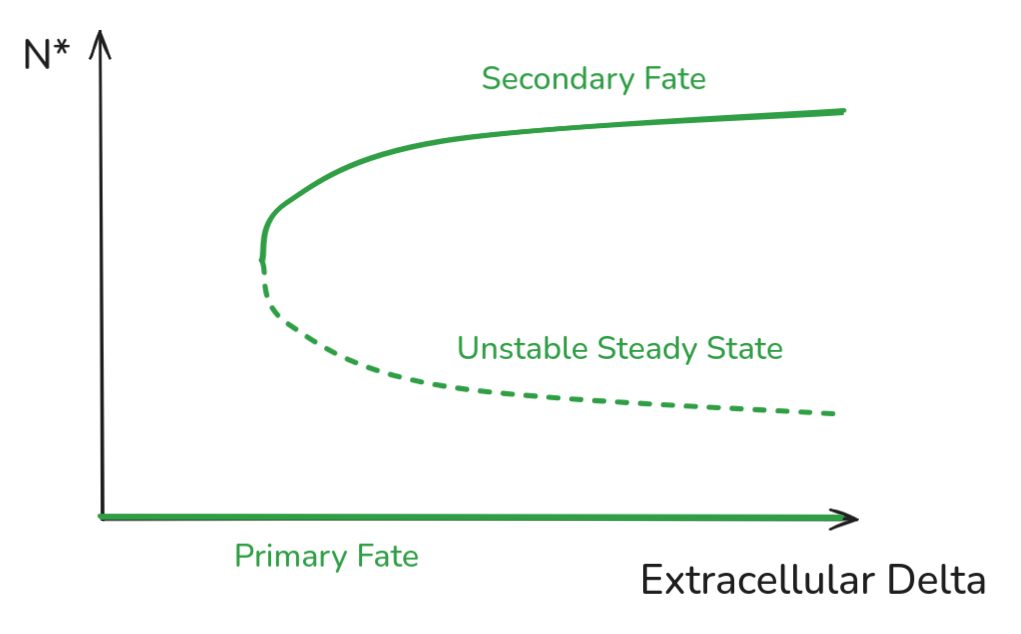
\includegraphics[width=\textwidth]{bifurcation-diagram}

\end{flushleft}

\end{document}







